\chapter{{\TeX}nik und Typographie}\label{ch-tech}

Die grundsätzliche Philosophie von \LaTeX\ ist, dass sich die Autoren auf den
Inhalt konzentrieren und um das Erscheinungsbild des Textes keine großen
Gedanken machen sollen.  Die typographischen "Entscheidungen", die das System
bzw.\ die Dokumentenklasse trifft, sind in der Regel sinnvoll und führen zu
besseren Ergebnissen als manuelle Eingriffe ungeübter Benutzer.

Wenn Sie sich dabei erwischen, dass Sie Abstände, Positionen, Größen oder
andere Parameter manipulieren, dann machen Sie sehr wahrscheinlich etwas
falsch.  (Eine Ausnahme sind Dinge wie die Titelseite, die einer Vorgabe
nachempfunden werden sollen.)

In diesem Kapitel werden einige \textit{Best Practices} aufgeführt, die
besonders die Leser aufmerksam studieren sollten, die noch nicht so erfahren
im Umgang mit \LaTeX\ sind.  Auf diverse typische Fehler im Umgang mit \LaTeX\
weist das Video \url{https://youtu.be/OSzs9K6-fRQ} hin, aber es ist kein
Ersatz für ein einführendes Buch.

\section{Verwendung der Vorlage}

Die Vorlage setzt ein installiertes \TeX-System wie
\href{https://de.wikipedia.org/wiki/MiKTeX}{\textsc{MiK\TeX}} oder
\href{https://de.wikipedia.org/wiki/TeX_Live}{\textsc{\TeX\ Live}} voraus.
Sie ist für das Kompilieren mit
\href{https://de.wikipedia.org/wiki/LuaTeX}{\textsc{Lua\TeX}} gedacht (und
wird daher mit \href{https://de.wikipedia.org/wiki/PdfTeX}{\textsc{pdf\TeX}}
nicht ohne entsprechende Änderungen funktionieren).  Die Bibliographie wird
mit \href{https://en.wikipedia.org/wiki/Biber_(LaTeX)}{\textsc{Biber}}
bearbeitet.

Es ist nicht möglich, in diesem Rahmen für jede Entwicklungsumgebung die
richtigen Optionen anzugeben.  Daher nur Anmerkungen zu drei weitverbreiteten
Tools:\footnote{Die ExpertInnen wissen natürlich, wie man so etwas
  automatisieren kann.}
\begin{itemize}
\item Für \href{https://de.wikipedia.org/wiki/TeXstudio}{{\TeX}studio} muss
  man in der Konfiguration als \textit{Standardcompiler} die Option
  \texttt{LuaLaTeX} auswählen und als \textit{Standard Bibliographieprogramm}
  die Option \texttt{Biber}.
\item Für \href{https://de.wikipedia.org/wiki/TeXworks}{{\TeX}works} benötigt
  man einen Durchlauf mit der Einstellung \texttt{LuaLaTeX} und dann einen mit
  der Einstellung \texttt{Biber}.  Danach lässt man das Dokument noch einmal
  mit der Einstellung \texttt{LuaLaTeX} kompilieren und kann in dieser
  Einstellung bleiben.  Einen weiteren \texttt{Biber}-Durchlauf zwischendurch
  benötigt man nur dann, wenn in der Bibliographie etwas geändert wurde.
\item Wenn Sie \href{https://www.ctan.org/pkg/latexmk/}{\textsc{latexmk}}
  benutzen, dann können Sie die Vorlage einfach mit
  \begin{center}
    \verb|latexmk -lualatex -bibtex VorlageBA.tex|
  \end{center}
  kompilieren und alles sollte ohne weiteren Eingriff funktionieren.
\end{itemize}

Nach diesen Schritten sollte das erzeugte PDF exakt so aussehen wie das, das
Sie gerade lesen.  Die Vorlage besteht aus mehreren Dateien, die in
Tabelle~\ref{tab-files} auf Seite~\pageref{tab-files} aufgeführt sind.  Für
einen kurzen Text wie diesen könnte man zur Not auch mit einer Datei
auskommen, aber für umfangreichere Dokumente ist eine Aufteilung nach diesem
Muster empfehlenswert.  Für \textsc{Lua\TeX} müssen die Quelldateien (also die
mit der Endung \texttt{.tex})
\href{https://de.wikipedia.org/wiki/UTF-8}{UTF-8}-kodiert sein.  Die Vorlage
ist als Gerüst für Ihre Arbeit gedacht und als Vorschlag zu betrachten.  In
den meisten Fällen gibt es alternative Methoden, um zu vergleichbaren
Ergebnissen zu kommen.  Wenn Sie sich gut mit \LaTeX\ auskennen, spricht
nichts dagegen, beispielsweise andere Pakete, andere Befehle oder andere
Optionen zu verwenden.

Die Dateien sind mit ausführlichen Kommentaren versehen.  Viele Informationen
zur Verwendung der Vorlage finden Sie nur in diesen Kommentaren und
\textit{nicht} in dem Text, den Sie gerade lesen!

Die Datei, die kompiliert werden muss und die die anderen lädt, ist
\texttt{VorlageBA.tex}.  Diese Datei sollten Sie zunächst umbenennen (z.\,B.\
in \texttt{BANameVorname.tex}), damit das erzeugte PDF-Dokument keinen
generischen Namen hat, sondern Ihnen zugeordnet werden kann.  Wenn Sie die
anderen Dateien umbenennen, dann müssen in den entsprechenden Aufrufen von
Befehlen wie \verb|\include| oder \verb|\addbibresource| auch die Namen
angepasst werden.

\section{Textformatierung}

In der Vorlage sind, abgesehen von der Titelseite, die freien Schriftarten
\href{https://tug.org/FontCatalogue/libertinusserif/}{\textit{Libertinus}} für
Fließtext und
\href{https://tug.org/FontCatalogue/anonymouspro/}{\textit{Anonymous Pro}} für
Code in einer Größe von 12~Punkt eingestellt.  Diese Schriften sind im Druck
und auf dem Bildschirm gut lesbar und aufeinander abgestimmt.  Außerdem bietet
diese Kombination volle Unterstützung für mathematischen Formelsatz.  Wenn Sie
kein Experte für Typographie sind, sollten sie keine Zeit damit verschwenden,
andere Schriftsätze auszuprobieren.  Der Zeilendurchschuss ist etwas
großzügiger bemessen, als man es für den Druck eines Buches machen würde.
Auch diesen Parameter sollten Sie nicht ohne triftigen Grund ändern.

\section{Mehrsprachiger Text}

Die Vorlage ist für Text in deutscher Sprache angelegt, in dem auch englische
Zitate vorkommen können.  Dafür wird das Standardpaket
\href{https://www.ctan.org/pkg/babel}{\textsc{babel}} eingesetzt.  Damit die
automatische Silbentrennung sowie einige andere Details richtig funktionieren,
muss \LaTeX\ "wissen", welche Sprache gerade verwendet wird.  Beispiele dafür,
wie man dem System den Wechsel der Sprache mitteilt, findet man in den Dateien
\texttt{chap3.tex} und \texttt{title.tex}.
Weitere Sprachen kann man in der Datei \texttt{defs.tex} hinzufügen.

% An dieser Stelle wird eine Möglichkeit, die Sprache zu wechseln, gezeigt.
% Beachten Sie, dass der gesamte Bereich zusätzlich durch { und } abgetrennt
% ist.  Das ist nötig, damit auch danach noch " (siehe \MakeOuterQuote{"} in
% defs.tex) funktioniert.
{
  \begin{otherlanguage}{english}
    This paragraph only serves to demonstrate that "quotation marks" will be
    treated correctly depending on the choice of language.
  \end{otherlanguage}
}

\section{PDF-Ausgabe}

Wenn Sie die Vorlage wie vorgesehen verwenden, werden durch das Paket
\href{https://ctan.org/pkg/hyperref}{\textsc{hyperref}} automatisch
Lesezeichen zur bequemen Navigation in den gängigen PDF-Programmen gesetzt.
Außerdem können (und sollten) dem Dokument auch Metadaten zugewiesen werden.
Dies geschieht am Ende der Datei \texttt{defs.tex}.  Dort müssen Sie Ihren
Namen und den Titel Ihrer Arbeit eingeben.
Ebenfalls am Ende von \texttt{defs.tex} wird erklärt, wie Sie
\textsc{hyperref} so umkonfigurieren, dass für die gedruckte Version Ihrer
Arbeit Links nicht farbig dargestellt werden.

\section{Verweise}

\subsection{Querverweise}\label{sec-ref}

Wenn Sie für Querverweise auf Abschnitte, Formeln, Seiten, Abbildungen usw.\
die Standardbefehle \verb|\label|, \verb|\ref|, \verb|\eqref| und
\verb|\pageref| benutzen, sorgt \LaTeX\ automatisch dafür, dass alles richtig
nummeriert wird und im PDF zusätzlich Links gesetzt werden.  In der Vorlage
finden Sie diverse Beispiele für den Einsatz dieser Befehle.  Sie sollten
Querverweise auf keinen Fall manuell in der Form "\texttt{siehe Kapitel~3}"
oder "\texttt{auf Seite~42}" eintippen!

\subsection{Zitate und Literaturverweise}\label{sec-litref}

% Im folgenden Absatz finden Sie verschiedene Varianten des Zitierbefehls
% \cite.  Außerdem wird gezeigt, wie man selbst steuern kann, welche Art der
% Nummerierung die Umgebung "enumerate" verwendet.  Siehe dazu die Anleitung für
% das Paket "enumitem".
Bei Verweisen auf die Literatur werden immer Autor und Jahr angegeben,
typischerweise in der Form \parencite{weitz2}.  Wörtliche Zitate werden
zusätzlich durch Anführungszeichen oder durch kursive Schrift gekennzeichnet
und mit der Seitenzahl versehen.  Es folgen ein paar Beispiele:
\begin{enumerate}[label=(\roman*)]
  % Die folgenden Zeilen zeigen, dass man auch einzelne Aufzählungspunkte
  % mit \label markieren kann, so dass man mit \ref auf sie verweisen kann.
\item\label{it-rec-a} Man kann die Leibnizformel mit zahlentheoretischen Methoden herleiten.
  Das ist allerdings relativ umständlich \parencite{weitz}.
\item Wie \citeauthor{weitz} in (\citeyear{weitz}) schreibt, kann man die
  Leibnizformel mit zahlentheoretischen Methoden herleiten.  Das sei
  allerdings relativ umständlich
  % Beachten sie die beiden leicht abweichenden Methoden der Verwendung von
  % \foreignlanguage:
\item\label{it-rec-b} Das Fazit des Autors nach Abwägen aller Alternativen:
  \foreignlanguage{english}{"The crux of the biscuit is the
    apostrophe"} \parencite[S.\ 42]{zappa}.\footnote{Hier werden die
    Anführungszeichen des fremdsprachlichen Zitates verwendet, während im
    nächsten Beispiel deutsche Anführungszeichen um den fremdsprachlichen Text
    herum benutzt werden.  Insbesondere für kurze Zitate in anderen Sprachen
    gibt es dafür keine einheitlichen Regeln.  Sie sollten aber zumindest
    konsistent vorgehen und im gesamten Dokument nur eine von beiden
    Alternativen verwenden.}
\item \citeauthor{zappa} kommt in (\citeyear{zappa}) schließlich und endlich
  zum Ergebnis: "\foreignlanguage{english}{The crux of the biscuit is the
    apostrophe}" (S.\ 42).
\item\label{it-foot} Man kann die Leibnizformel mit zahlentheoretischen Methoden herleiten.
  Das ist allerdings relativ umständlich.\footcite{weitz}
\end{enumerate}
Die Versionen \ref{it-rec-a} und~\ref{it-rec-b} sind am übersichtlichsten
und werden empfohlen.  Die Alternative~\ref{it-foot} --~Quellenangaben in den
Fußnoten~-- ist für Bachelorarbeiten in unserem Department eher unüblich und
sollte nur nach Absprache verwendet werden.

\section{Mathematische Formeln}

Mathematischer Formelsatz ist die Spezialität von \LaTeX.  Während man
allerdings Texte in \LaTeX\ fast so wie in einem Textverarbeitungsprogrammen
schreiben kann, muss man für Formeln eine eigene Sprache lernen.  Einen
"Crashkurs" für diese mathematische Syntax, die man inzwischen auch in
\textsc{Word} und vielen anderen Programmen verwenden kann, bietet das Video
\url{https://youtu.be/7ovgNXRiJ6g}.  (Siehe auch das am Anfang von
Kapitel~\ref{ch-tech} erwähnte Video zu typischen Fehlern.)  Auch hier gilt
aber die Anmerkung, dass ein Lehrbuch die bessere Quelle sein wird.

% Die Umgebung "equation" brauchen Sie nur, wenn Sie sich später auf die
% Formel beziehen wollen.  Der dazu gedachte Befehl \eqref wird weiter unten
% exemplarisch verwendet.  Das Paket "amsmath" bietet viele weitere Umgebungen
% (mit und ohne Nummerierung), z.B. für mehrzeilige Formeln.
Die Vorlage ist so eingerichtet, dass eingerückte Formeln nicht zentriert
werden, sondern wie beispielsweise
\begin{equation}
  \int_a^b g(t)\,\mathrm{d}t = \int_a^b \Re(g(t))\,\mathrm{d}t + \mathrm{i}\int_a^b \Im(g(t))\,\mathrm{d}t\label{eq-integ}
\end{equation}
etwas versetzt am linken Rand anfangen.  Diese Einstellung kann man beim
Aufruf des Befehls \verb|\documentclass| ändern, indem man die Option
\verb|fleqn| entfernt.

% Hier sehen Sie "normale" Formeln (ohne Nummerierung) sowohl im Fließtext als
% auch abgesetzt.
Im mathematischen Kontext ist es üblich, dass Formeln wie Satzbestandteile der
normalen Sprache behandelt werden.  Das hat insbesondere Auswirkungen auf die
Interpunktion.  Zum Beispiel besagt die verallgemeinerte Kontinuumshypothese,
dass für jede Ordinalzahl $\alpha$ die Gleichung
$\aleph_\alpha = \beth_\alpha$ gilt.  In der Sprache der
Zermelo-Fraenkel-Mengenlehre heißt das
\[ \forall \alpha \in \operatorname{ON} \; 2^{\aleph_\alpha} =
  \aleph_{\alpha+1}. \] Dieses Beispiel sollte nur demonstrieren, dass hier an
das Ende der Formel ein Punkt gehört, weil der Satz dort endet.
Abgesetzte Formeln wie die gerade gezeigte sollten normalerweise nicht
nummeriert werden.  Eine Ausnahme davon sind natürlich Formeln
wie~\eqref{eq-integ}, auf die später mit \verb|\eqref| verwiesen wird.

Die Vorlage lädt automatisch die Erweiterung
\href{https://de.wikipedia.org/wiki/AMS-LaTeX}{\AmS-\LaTeX}, die viele
hilfreiche Erweiterungen für mathematische Ausdrücke enthält.  Ohne dieses
Paket wäre es beispielsweise wesentlich aufwendiger, Kettenbrüche wie
\[ \mathrm{e} = \sum_{k=0}^\infty \frac1{k!} = \lim_{n\to\infty} \Bigl(1+\frac1n\Bigr)^n = 2 + \cfrac{1}{1 
    + \cfrac{1}{2 
      + \cfrac{2}{3
        + \cfrac{3}{4
          + \cfrac{4}{5
            + \cfrac{5}{\ddots
      } } } } } } \]
darzustellen.

\section{Elemente in Gleitumgebungen}\label{sec-float}

Tabellen und Abbildungen sollten grundsätzlich mit einer Beschriftung
(\verb|\caption|) versehen sein.  Dazu gehört auch eine Quellenangabe, wenn es
sich um Daten handelt, die Sie übernommen haben.  Außerdem sollten solche
Objekte immer in eine sogenannte Gleitumgebung wie \texttt{table} oder
\texttt{figure} gesetzt werden, damit \LaTeX\ für eine richtige Platzierung
sorgen kann und die Objekte ggf.\ in Verzeichnissen (siehe
Abschnitt~\ref{sec-lists}) erfasst werden können.  Viel mehr zu diesem Thema
findet man u.\,a.\ in \parencite[Kap.\ 11]{voss}.

In der Vorlage stehen Beschriftungen für Tabellen und Codeblöcke (siehe
Abschnitt~\ref{sec-code}) jeweils links eingerückt über den Tabellen und
Beschriftungen für Abbildungen zentriert unter diesen.  Achten Sie darauf, den
\verb|\caption|-Befehl entsprechend am Anfang bzw.\ am Ende der Gleitumgebung
aufzurufen.

\subsection{Tabellen}

Für typographisch anspruchsvoll gesetzte Tabellen verwendet die Vorlage das
Paket \href{https://www.ctan.org/pkg/booktabs}{\textsc{booktabs}} zusammen mit
der Standardumgebung \texttt{tabular}.  Beispiele für Tabellen finden Sie in
den Dateien \texttt{chap2.tex} und \texttt{chap3.tex}.  Grundsätzlich gilt,
dass Linien in Tabellen im Allgemeinen \textit{nicht} der Übersichtlichkeit
dienen, sondern bezüglich der Lesbarkeit kontraproduktiv sind.  In den meisten
Ratgebern zur Typographie wird insbesondere empfohlen, auf vertikale Linien
komplett zu verzichten!
In Tabelle~\ref{tab-fail} gibt es eher zu viele Linien.  Die wurden dort
lediglich eingefügt, um ein paar Gestaltungsmöglichkeiten von
\textsc{booktabs} zu demonstrieren.

% Ein kommentiertes Beispiel für eine Tabelle befindet sich bereits in
% chap2.tex.  Hier sei nur noch auf den Befehl \cmidrule für "Teilstriche"
% hingewiesen.
\begin{table}[!ht]
  \caption{Durchfallquoten Mathematik}
  \centering
  \begin{tabular}{lrrrr}
    \toprule
    \textit{\color{gray}Fantasiewerte!}&Jahr&&& \\[-2pt]
    &2018&2019&2020&2021 \\
    \cmidrule(lr){2-2}
    \cmidrule(lr){3-3}
    \cmidrule(lr){4-4}
    \cmidrule(lr){5-5}
    Sommersemester&16{,}5\,\%&15{,}4\,\%&14{,}3\,\%&13{,}2\,\%\\
    Wintersemester&26{,}5\,\%&25{,}4\,\%&24{,}3\,\%&23{,}2\,\%\\
    \cmidrule[0.8pt](lr){1-1}
    \cmidrule(lr){2-2}
    \cmidrule(lr){3-3}
    \cmidrule(lr){4-4}
    \cmidrule(lr){5-5}
    Gesamt&21{,}5\,\%&20{,}4\,\%&19{,}3\,\%&18{,}2\,\%\\
    \bottomrule
  \end{tabular}
  \label{tab-fail}
\end{table}

Rein technisch ist es möglich, mit \verb|\includegraphics| Tabellen
einzufügen, die in anderen Programmen erzeugt wurden.  Das sollte aber
eigentlich immer vermieden werden, weil es sehr häßlich aussieht.  Siehe dazu
auch die Anmerkungen in Abschnitt~\ref{sec-fig}.
Für Tabellen, die länger als eine Seite sind, werden spezielle Pakete wie
beispielsweise \href{https://ctan.org/pkg/longtable}{\textsc{longtable}}
benötigt.

Es gibt diverse Tools, die Daten aus Programmen wie \textsc{Excel} einlesen
und diese in \LaTeX-Syntax als Tabellen ausgeben können.  Manche Programme,
z.\,B.\ \textsc{Mathematica}, können auch direkt nach \LaTeX\ exportieren.

\subsection{Abbildungen}\label{sec-fig}

Abbildungen können mit dem Befehl \verb|\includegraphics| eingefügt werden.
Wenn es sich nicht um Fotos handelt, ist jedoch darauf zu achten, dass auf
jeden Fall skalierbare Vektorgrafiken verwendet werden.  Rastergrafiken (wie
sie beispielsweise durch Screenshots oder Scans erzeugt werden) führen,
insbesondere im Druck, fast immer zu suboptimalen Ergebnissen.  Das wird etwas
übertrieben in Abbildung~\ref{fig-bad} dargestellt.

% Ein Beispiel für eine Abbildung; die Abbildung selbst wird mit dem
% Befehl \includegraphics geladen.  Die Umgebung \figure sorgt u.a. für das
% "Gleiten" und die Aufnahme in das Abbildungsverzeichnis.
\begin{figure}[!ht]
  % Zentrieren der Abbildung
  \centering
  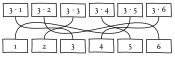
\includegraphics[width=.8\textwidth]{bitmap}
  % Beschriftung der Abbildung; in eckigen Klammern der Titel für das
  % Abbildungsverzeichnis
  \caption[Schlecht: Rastergrafik]{Ganz schlechtes Beispiel! (Quelle: \cite[S. 184]{weitz})}
  % frei wählbarer Name für \ref
  \label{fig-bad}
\end{figure}

Abbildung~\ref{fig-better} zeigt im Vergleich eine Vektorgrafik.  Das ist
schon besser, hat aber in den meisten Fällen den Nachteil, dass die Schriften
nicht mit denen Ihrer Arbeit übereinstimmen werden, was unter typographischen
Aspekten sehr unschön ist.\footnote{Das gilt "erst recht" für Tabellen, die
  aus externen Quellen eingefügt werden.}  (Der zugehörige Code in der Datei
\texttt{chap3.tex} zeigt nebenbei, wie man eingefügte Grafiken beschneiden
kann.)

\begin{figure}[!ht]
  \centering
  % es wird nur ein Ausschnitt des Originals eingetzt; die Reihenfolge der
  % vier Werte ist: left bottom right top
  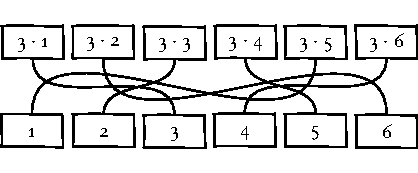
\includegraphics[width=.8\textwidth,trim={0mm 4mm 0mm 4mm},clip]{vector}
  \caption[Besser, aber noch nicht gut: Vektorgrafik]{Besser, aber nicht optimal (Quelle: \cite[S. 184]{weitz})}
  \label{fig-better}
\end{figure}

Die beste Lösung ist das Erstellen der Grafiken direkt in \LaTeX.  Dazu eignet
sich hervorragend das Paket
\href{https://de.wikipedia.org/wiki/PGF/TikZ}{\textsc{PGF/Ti\textit{k}Z}}, das
nahezu unbegrenzte Möglichkeiten bietet, jedoch eine steile Lernkurve hat.
Dafür ist die mitgelieferte Dokumentation allerdings auch hervorragend.  Als
Einführung kann man auch die Videos in der Playlist
\begin{center}
\url{https://www.youtube.com/playlist?list=PLb0zKSynM2PBbpe9x6LgOZkSCl2yJAOQY}
\end{center}
verwenden.

Diese Vorgehensweise hat zudem den Vorteil, dass man potentiellen Problemen
mit dem Urheberrecht aus dem Weg geht, weil dieses nicht auf eine nach einer
Vorlage selbst erstellte Grafik anwendbar ist.  Nichtsdestotrotz muss aber
auch in diesem Fall die Herkunft benannt werden!

% Zwei ausführliche Beispiele für die Verwendung von TikZ; siehe dazu die
% verlinkte YouTube-Playlist sowie die sehr empfehlenswerte
% TikZ-Dokumentation.
\begin{figure}[!ht]
  \centering
    \begin{tikzpicture}[scale=1.5]
      \useasboundingbox (-.5,-.5) rectangle (4.5,6.5);
      \coordinate (O) at (0,0);
      \coordinate (A) at (4,0);
      \coordinate (B) at (4,6);
      \coordinate (E) at (0,6);
      \path[name path=rightEdge] (4,0) -- (B);
      \path[name path=firstHypo] (O) -- ($(O)!1.5!35:(A)$);
      \path[name intersections={of=rightEdge and firstHypo}] (intersection-1) coordinate (C);
      \path[name path=topEdge] (B) -- (E);
      \path[name path=sinEdge] (C) -- ($(C) + (125:5)$);
      \path[name intersections={of=topEdge and sinEdge}] (intersection-1) coordinate (D);
      \fill[haw3] (O) -- (A) -- (C) -- cycle;
      \fill[haw2, fill opacity=.5] (O) -- (C) -- (D) -- cycle;
      \draw (O) rectangle (4,6);
      \draw (O) -- node[sloped, above] {$\cos\beta$} (C);
      \draw (C) -- node[sloped, below] {$\sin\beta$} (D);
      \path (O) -- node[sloped, above] {$\sin(\alpha+\beta)$} (E);
      \path (O) -- node[sloped, below] {$\cos\alpha\,\cos\beta$} (A);
      \path (C) -- node[rotate=180, sloped, above] {$\sin\alpha\,\cos\beta$} (A);
      \path (B) -- node[sloped, above] {$\cos\alpha\,\sin\beta$} (C);
      \path (E) -- node[sloped, above] {$\cos(\alpha+\beta)$} (D);
      \path (D) -- node[sloped, above] {$\sin\alpha\,\sin\beta$} (B);
      \draw (O) -- (C);
      \draw (C) -- (D);
      \draw[ultra thick] (D) -- node[above left, xshift=1mm] {\Large$\mathbf{1}$} (O);
      \draw pic[pic text={\small$\alpha$}, angle radius=1.4cm, draw=black] {angle=A--O--C};
      \draw pic[pic text={\small$\beta$}, angle radius=1.4cm, draw=black] {angle=C--O--D};
      \draw pic[pic text={\small$\alpha+\beta$}, angle radius=1.4cm, draw=black] {angle=E--D--O};
      \draw pic[pic text={\small$\alpha$}, angle radius=1.4cm, draw=black] {angle=B--C--D};
    \end{tikzpicture}
  \caption[Erstes \textsc{Ti\textit{k}Z}-Beispiel]{Mit \textsc{Ti\textit{k}Z} [eigene Grafik nach \parencite[S. 271]{weitz}]}
  \label{fig-tikz}
\end{figure}

% ein Hilfsbefehl für die folgende TikZ-Grafik
\newcommand{\foo}[5]{
  \begin{scope}[xshift=#1cm]
    \begin{scope}[x  = {(1cm,0cm)}, y  = {(0.4cm,0.6cm)}, z  = {(0cm,1cm)}]
      \begin{scope}[canvas is xz plane at y=#4]
        \filldraw[black, fill=#3!70!white] ($(0,0) + (0,#5)$) rectangle ($(0.5,#2) + (0,#5)$);
      \end{scope}
      \pgfmathsetmacro{\z}{#2 + #5}
      \begin{scope}[canvas is xy plane at z=\z]
        \filldraw[black, fill=#3!50!white] (0,#4) -- (0.5,#4) -- ($(0.5,1) + (0,#4)$) -- ($(0,1) + (0,#4)$) -- cycle;
      \end{scope}
      \begin{scope}[canvas is yz plane at x=0.5]
        \filldraw[black, fill=#3!90!white] (#4,#5) rectangle ($(1,#2) + (#4,#5)$);
      \end{scope}
    \end{scope}
  \end{scope}
}

Die Abbildungen \ref{fig-tikz} und~\ref{fig-tikz2} zeigen Beispiele für solche
Grafiken.  Den zugehörigen Quellcode findet man in der Datei
\texttt{chap3.tex}.

\begin{figure}[!ht]
  \centering
    \begin{tikzpicture}[scale=1.5]
      \foreach \i in {1, ..., 16} {
        \pgfmathsetmacro{\shift}{\i / 2}
        \pgfmathsetmacro{\height}{6 / \i}
        \foo{\shift}{\height}{gray}{0}{0}
      }
      \foo{0.5}{3}{haw2}{-1}{0}
      \foo{0.5}{3}{haw3}{-1}{3}
      \foo{1}{3}{haw}{-1}{0}
      \foo{1.5}{1.5}{orange}{-1}{0}
      \foo{2}{1.5}{orange}{-1}{0}
      \foo{2.5}{.75}{purple}{-1}{0}
      \foo{3}{.75}{purple}{-1}{0}
      \foo{3.5}{.75}{purple}{-1}{0}
      \foo{4}{.75}{purple}{-1}{0}
      \foreach \i in {1, ..., 8} {
        \pgfmathsetmacro{\x}{4 + 0.5 * \i}
        \foo{\x}{.375}{brown}{-1}{0}
      }
    \end{tikzpicture}
  \caption[Zweites \textsc{Ti\textit{k}Z}-Beispiel]{Auch mit \textsc{Ti\textit{k}Z} [eigene Grafik nach \parencite[S. 533]{weitz}]}
  \label{fig-tikz2}
\end{figure}

\section{Code}\label{sec-code}

Für die Darstellung von Programmcode wie in Codeblock~\ref{euler} wird in der
Vorlage das Paket \href{https://www.ctan.org/pkg/listings}{\textsc{listings}}
verwendet.

% Verwendung des Pakets "listings" für die Darstellung von Code, der aus der
% externen Datei euler.py gelesen wird
\lstinputlisting[
% das Paket "kennt" viele gängige Programmiersprachen
    language=Python,
% Beschriftung
    caption=Eulersches Polygonzugverfahren,
% frei wählbarer Name für \ref
    label=euler
]{euler.py}

In der Datei \texttt{chap3.tex} kann man sehen, wie der Code aus einer
externen Datei eingelesen wird.  Durch diese Vorgehensweise kann man dafür
sorgen, dass auch tatsächlich die aktuelle Version des eigenen Codes verwendet
wird, und man vermeidet potentielle Fehler beim Abtippen.  Man kann den Code
aber auch wie in Codeblock~\ref{kperms} direkt eintippen.

% Verwendung des Pakets "listings" für die Darstellung von Code, der direkt im
% LaTeX-Code eingegeben wird
\begin{lstlisting}[language=Python,caption=Variationen,label=kperms]
def kperm(L, k):
    if k == 0:
        return [[]]
    return [[L[i]]+P for i in range(len(L))
                     for P in kperm(L[:i] + L[i+1:], k-1)]  
\end{lstlisting}

In der Datei \texttt{defs.tex} wird exemplarisch gezeigt, wie man das Aussehen
der Codeblöcke individuell gestalten kann.  Es ist auch möglich, Codeblöcke
wie Abbildungen und Tabellen "gleiten" zu lassen.

Ein Verzeichnis der Codeblöcke kann mit dem Paket \textsc{listings} bei Bedarf
erzeugt werden, wenn Ihre Arbeit sehr viele Codeblöcke enthält.  Umfangreiche
Codeblöcke gehören aber nicht in die Arbeit und auch nicht in den Anhang,
sondern sollten --~ggf. nach Absprache mit der Erstprüferin bzw.\ dem
Erstprüfer~-- auf einem Datenträger zusammen mit der Arbeit eingereicht
werden.